\clearpage
\section{Sampling of Truncated Recurrence}
\label{sec:sampling-truncated-recurrence}

\begin{figure}[!h]
\centering
\begin{minipage}[t]{0.48\textwidth}
\begin{algorithm}[H]
\caption{\textsc{\citet{geiping_scaling_2025}}}
\label{alg:poisson-fill}
\begin{algorithmic}[1]
\State \textbf{Input:} $\mu_{\text{rec}}$, $\mu_{\text{bwd}}, \Lambda$, $e$
\State $n \sim \Lambda(\mu_{\text{rec}} - \mu_{\text{bwd}})$
\State $k \gets \mu_{\text{bwd}}$
\State $T = n + k$
\State $h_0 \gets \mathcal{N}(0, \sigma^2 I)$
\For{$t = 1$ \textbf{to} $T$}
    \If{$t \leq n$}
        \State $h_t \gets \mathcal{R}(h_{t-1}, e)$ \textbf{w/o grad}
    \Else
        \State $h_t \gets \mathcal{R}(h_{t-1}, e)$ \textbf{w/ grad}
    \EndIf
\EndFor
\State \Return $x_T$
\end{algorithmic}
\end{algorithm}
\end{minipage}
\hfill
\begin{minipage}[t]{0.48\textwidth}
\begin{algorithm}[H]
\caption{\textsc{Correction (Ours)}}
\label{alg:poisson-trunc-full}
\begin{algorithmic}[1]
\State \textbf{Input:} $\mu_{\text{rec}}$, $\mu_{\text{bwd}}$, $\Lambda$, $e$
\State $T \sim \Lambda(\mu_{\text{rec}})$
\State $n \gets \max(T - \mu_{\text{bwd}}, 0)$
\State $k \gets \min(T, \mu_{\text{bwd}})$
\State $h_0 \gets \mathcal{N}(0, \sigma^2 I)$
\For{$t = 1$ \textbf{to} $T$}
    \If{$t \leq n$}
        \State $h_t \gets \mathcal{R}(h_{t-1}, e)$ \textbf{w/o grad}
    \Else
        \State $h_t \gets \mathcal{R}(h_{t-1}, e)$ \textbf{w/ grad}
    \EndIf
\EndFor
\State \Return $x_T$
\end{algorithmic}
\end{algorithm}
\end{minipage}
\caption{Comparison of our sampling method with \cite{geiping_scaling_2025}. It can be observed that the actual distribution of forward recurrence for \cite{geiping_scaling_2025} is a shifted Poisson distribution. The implications of this sampling strategy can be better visualized in \cref{fig:method-distribution-mismatch}.}
\label{fig:sampling-algos}
\end{figure}


\begin{figure}[h]
    \centering
    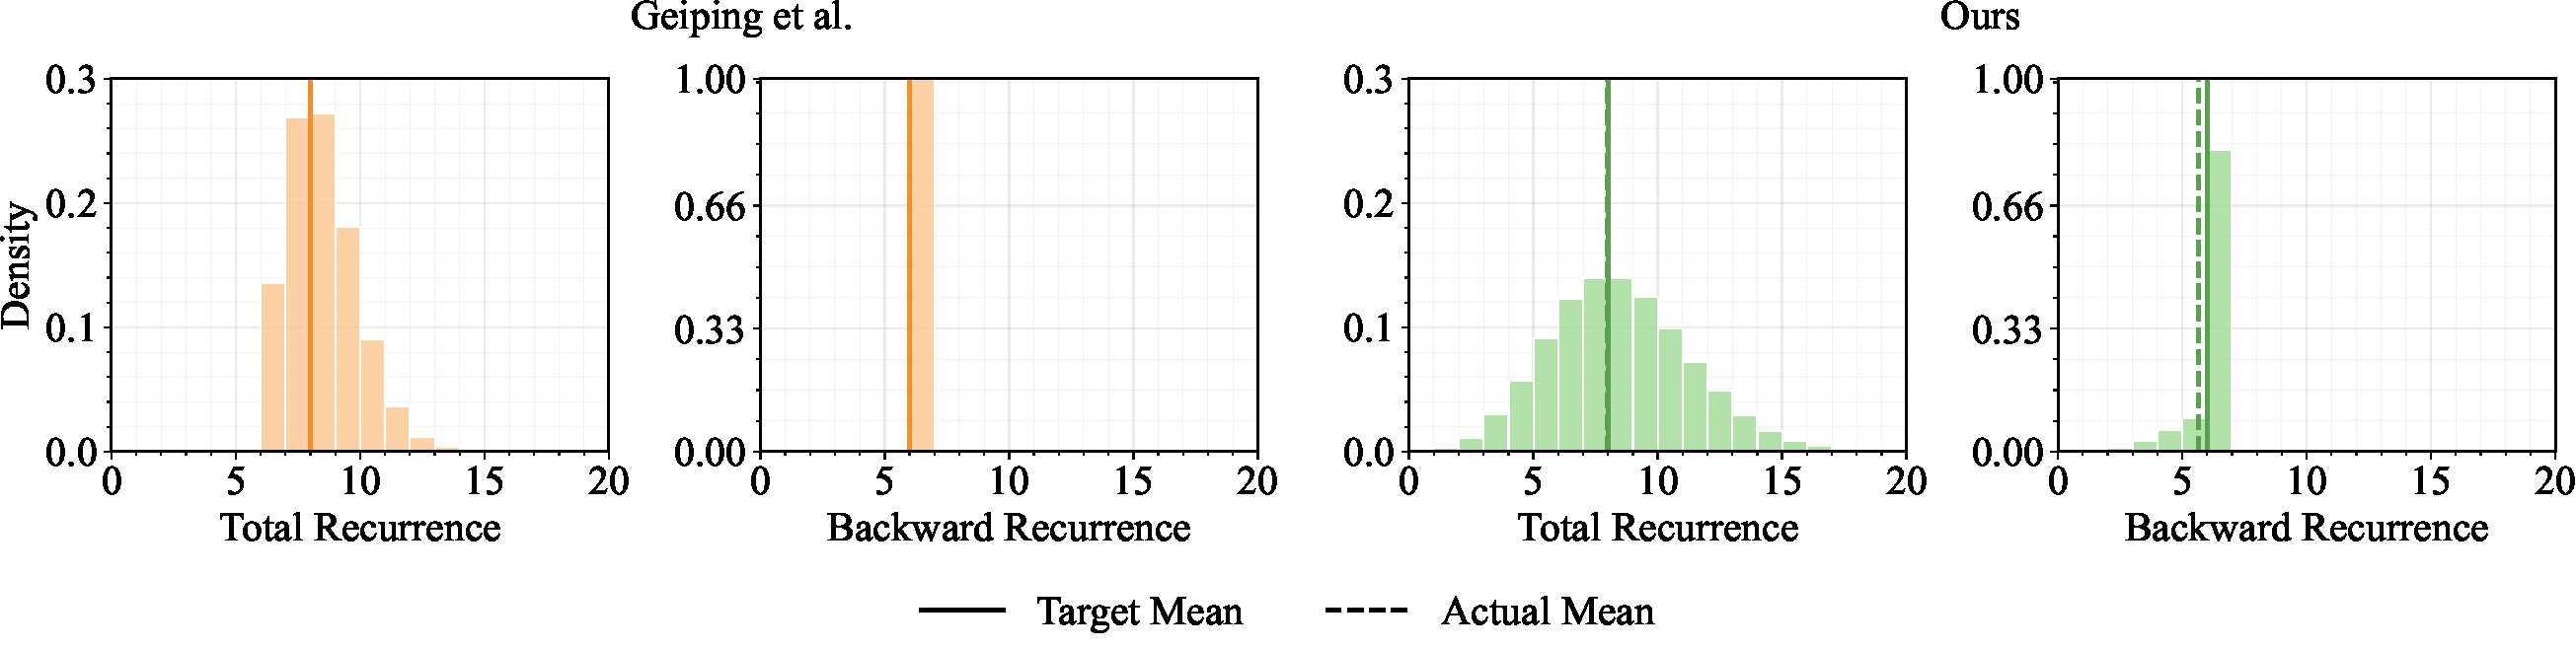
\includegraphics[width=\linewidth]{figures/appendix/distribution-mismatch.pdf}
    \caption{A distributional mismatch can be observed from the recurrent sampling method of \cite{geiping_scaling_2025}. Specifically, if our desired pre-training distribution for \meanrecurrence is a Poisson distribution, the distribution total recurrence $T$ of \cite{geiping_scaling_2025} is truncated based on \meanbackward. However, our sampling method decouples the effects of \meanbackward on $\Lambda$, allowing the recurrent distribution to be faithfully sampled from.}
    \label{fig:method-distribution-mismatch}
\end{figure}

In our very initial experiments, we observed that we could make a small change to the sampling algorithm of \cite{geiping_scaling_2025}, which stems from \cite{avi_learn_algorithm}, to enhance the training of Parcae\footnote{We make the same change to RDMs in the main body, observing that they perform better with it and to make comparison fair.}. When given an arbitrary distribution to sample from $\Lambda$ and two hyperparameters \meanrecurrence (the desired mean steps of the recurrent blocks in pre-training) and \meanbackward (the desired mean back-propagation steps in pre-training), we observe that previous work by \cite{geiping_scaling_2025} had a distributional mismatch. Previously, the sampling method of \cite{geiping_scaling_2025} exactly followed \cref{alg:poisson-fill} with a poisson log-normal distribution with the following distribution
\begin{align}
    \tau \sim \mathcal{N}(\log(\mu_{\text{rec}} - \mu_{\text{bwd}}) - \frac{1}{2}\sigma^2, \sigma) \qquad n \sim \mathcal{P}(e^\tau) + 1 \qquad k \gets \mu_{\text{bwd}}
\end{align}
where $\sigma = \frac{1}{2}$. To maintain a fixed computation memory budget, \cite{geiping_scaling_2025} sets $k$ to \meanbackward; however, this minor change significantly impacts the underlying recurrent distribution, truncating and compressing the distribution of recurrence actually observed during pre-training. We propose making a minor algorithmic fix to the sampling method, which can be observed in \cref{alg:poisson-trunc-full}. While minor, observe in \cref{fig:method-distribution-mismatch} the impact of improving generalization to other recurrences. 

To verify our change, we pretrain several small Parcae models on 10 billion tokens to ablate on our design choice. Specifically, we set $\mu_{\text{rec}} = \mu_{\text{bwd}} = 8$ and use $\Lambda \sim \text{Poisson}$, and use fixed architecture, hyperparameters, and data stream. We train three models: a baseline Parcae model that performs full backpropagation through recurrences, a Parcae model following \cref{alg:poisson-fill} by \cite{geiping_scaling_2025}, and a Parcae model following \cref{alg:poisson-trunc-full}. The results of this ablation can be found in \cref{fig:sampling-mismatch-results}.

\begin{figure}[t]
    \centering
    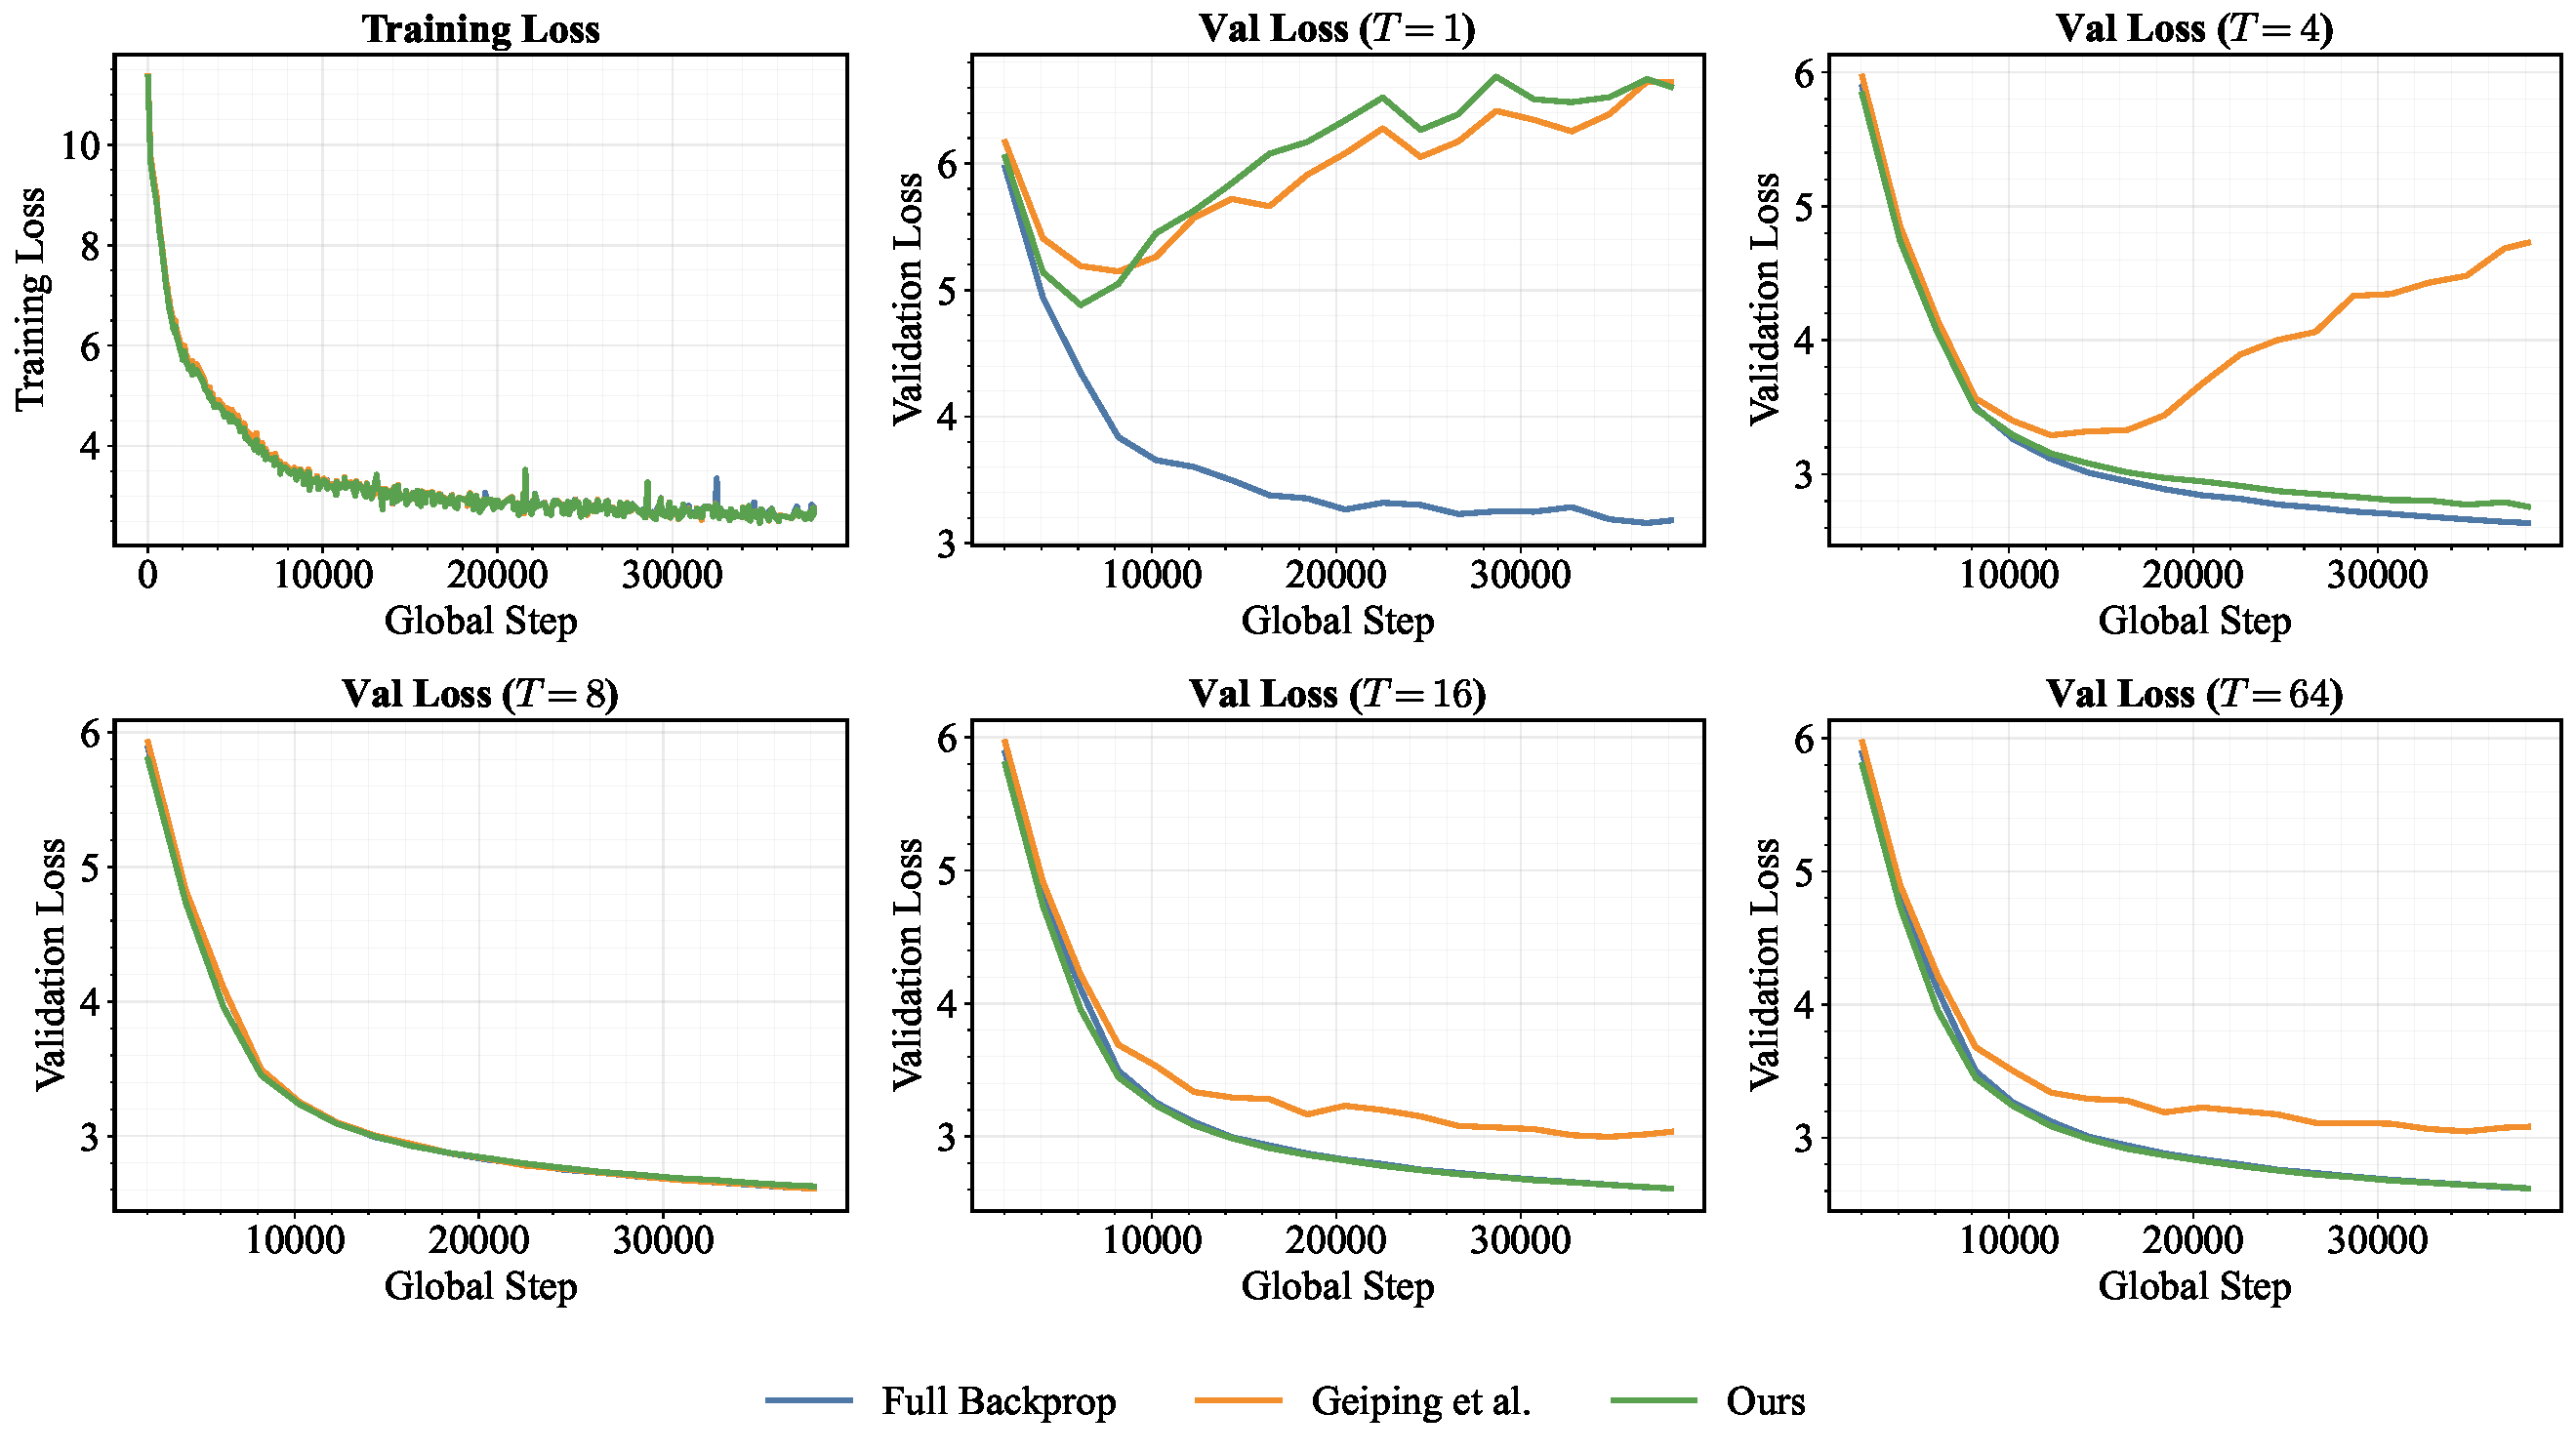
\includegraphics[width=\textwidth]{figures/appendix/loss_curves_publication.pdf}
    \caption{Training and validation curves of three 100 million parameter Parcae models pretrained on 10 billion tokens, comparing different truncated back-propagation methods (baseline is a model with no back-propagation truncation). Each model has identical architecture and hyperparameters, with \meanrecurrence and \meanbackward both being set to eight, all using $\Lambda \sim \text{Poisson}$. It can be observed that even though each model has similar training loss and validation loss when using $T=8$, our implementation more faithfully follows the validation loss of full back-propagation. Specifically for $T=4$, our implementation significantly improves validation loss compared to \cite{geiping_scaling_2025} sampling method.}
    \label{fig:sampling-mismatch-results}
    \vspace{-1em}
\end{figure}

From \cref{fig:sampling-mismatch-results}, observe that training trajectories and validation loss at $T=\mu_{\text{rec}}=8$ are almost identical for each run; however, our method significantly improves performance for the validation loss of $T \in [4,16,64]$. Simply put, the constricting effect \cite{geiping_scaling_2025} observed in \cref{fig:method-distribution-mismatch} reduces the effective range of recurrence seen in pretraining, hurting the validation loss of using more or fewer recurrence at test-time. 
